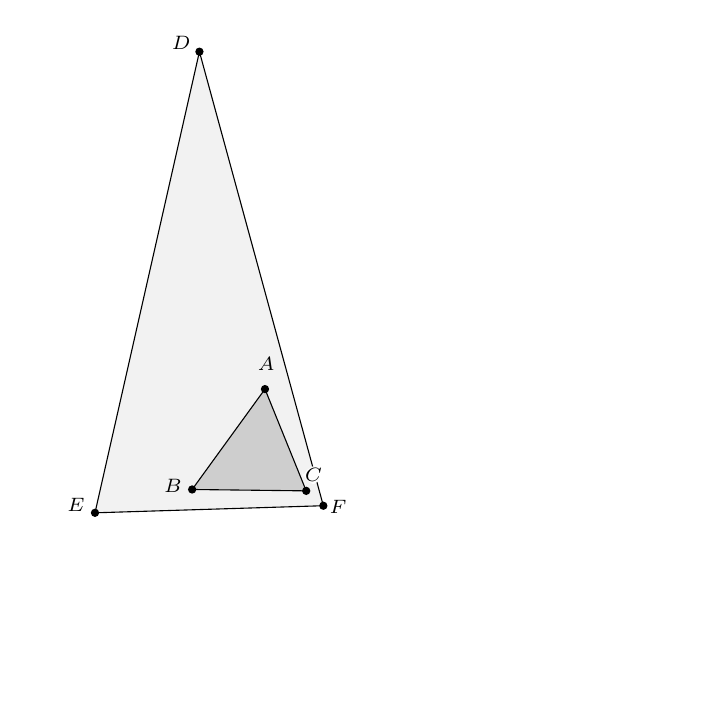
\begin{tikzpicture}[scale = 0.125]
    \clip(-22.59,-26.1) rectangle (44.94,41.07);
    \fill[fill=black,fill opacity=0.15] (1.52,4.35) -- (-5.88,-5.85) -- (5.71,-5.99) -- cycle;
    \fill[fill=black,fill opacity=0.05] (-5.14,38.63) -- (-15.75,-8.22) -- (7.45,-7.5) -- cycle;
    \draw (1.52,4.35)-- (-5.88,-5.85);
    \draw (-5.88,-5.85)-- (5.71,-5.99);
    \draw (5.71,-5.99)-- (1.52,4.35);
    \draw (-5.14,38.63)-- (-15.75,-8.22);
    \draw (-15.75,-8.22)-- (7.45,-7.5);
    \draw (7.45,-7.5)-- (-5.14,38.63);
    \begin{scriptsize}
        \fill [color=black] (1.52,4.35) circle (12pt);
        \draw[color=black] (1.64,6.88) node {$A$};
        \fill [color=black] (-5.88,-5.85) circle (12pt);
        \draw[color=black] (-7.84,-5.47) node {$B$};
        \fill [color=black] (5.71,-5.99) circle (12pt);
        \draw[color=black] (6.44,-4.39) node[fill = white, rounded corners = 5pt, inner sep=0.8pt] {$C$};
        \fill [color=black] (-5.14,38.63) circle (12pt);
        \draw[color=black] (-7,39.51) node {$D$};
        \fill [color=black] (-15.75,-8.22) circle (12pt);
        \draw[color=black] (-17.67,-7.39) node {$E$};
        \fill [color=black] (7.45,-7.5) circle (12pt);
        \draw[color=black] (8.95,-7.63) node {$F$};
    \end{scriptsize}
\end{tikzpicture}